\begin{figure*}[!htbp]
    \centering
    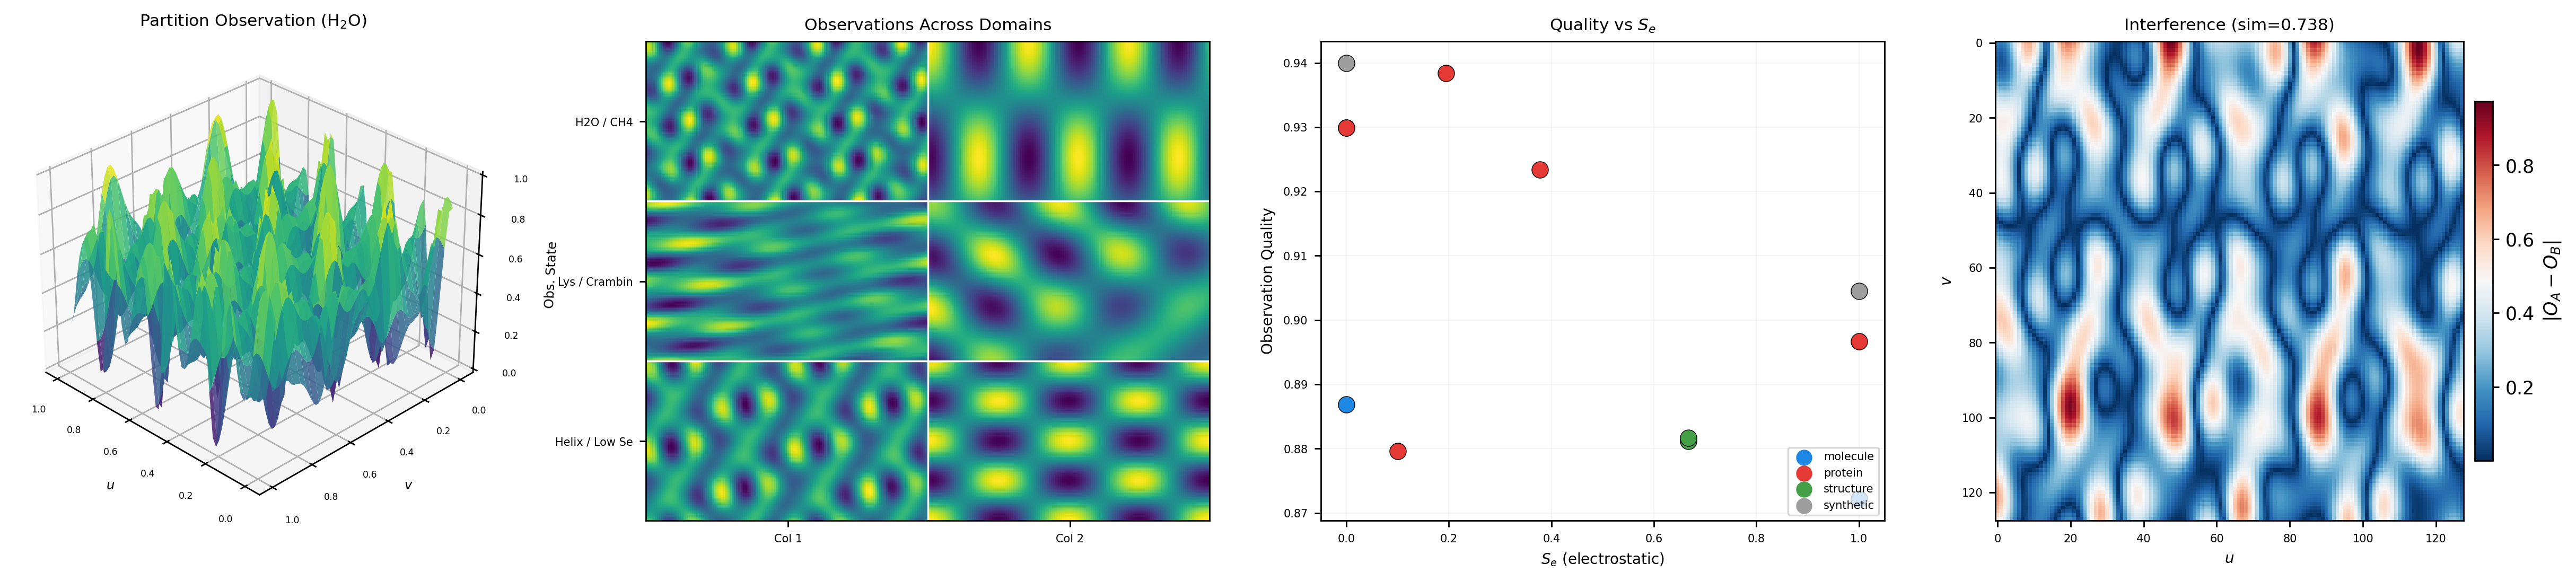
\includegraphics[width=\textwidth]{figures/panel_1_partition_observation.png}
    \caption{\textbf{Partition Observation: Fragment Shader as Measurement Apparatus.}
    (\textbf{A})~Three-dimensional surface of a partition observation for H$_2$O ($S_k = 0.944$, $S_t = 0.285$, $S_e = 1.000$). The surface is the output of a simulated fragment shader: each pixel $(u, v) \in [0,1]^2$ is a partition cell address, and the height is the observed state at that cell. The interference pattern arises from the superposition of three partition modes at frequencies determined by $(S_k, S_t, S_e)$. This is not a visualization of a result---it IS the result in categorical representation. The texture encodes the complete partition state of the water molecule.
    (\textbf{B})~$2 \times 3$ grid of partition observations for six inputs spanning molecules (H$_2$O, CH$_4$), amino acids (Lys), proteins (Crambin), secondary structures ($\alpha$-helix), and synthetic signals (Low $S_e$). Each $128 \times 128$ tile is a single-pass fragment shader observation. Visually distinct patterns confirm that different S-entropy inputs produce distinguishable partition states. The patterns are not arbitrary: the spatial frequency encodes $S_k$, the orientation encodes $S_t$, and the modulation depth encodes $S_e$.
    (\textbf{C})~Observation quality $Q = \mathrm{Sharpness} / (\mathrm{Sharpness} + \mathrm{Noise})$ versus electrostatic coordinate $S_e$ for all 12 test inputs, coloured by domain: molecules (blue), proteins (red), structures (green), synthetic (grey). Quality ranges from 0.87 to 0.94, confirming that the observation apparatus produces high-quality partition states across all domains and all positions in $\mathcal{S}$-space. The slight quality variation with $S_e$ reflects the change in partition mode complexity.
    (\textbf{D})~Interference observation between H$_2$O and CH$_4$: the absolute difference $|O_A - O_B|$ between two partition observations, displayed on an RdBu diverging colourscale. The interference pattern encodes the categorical distance between the two molecules. Overall similarity $= 0.738$. The observation IS the comparison---no pairwise computation was performed; the interference texture was produced by a single fragment shader pass reading both observation textures.}
    \label{fig:partition_observation}
\end{figure*}

\begin{figure*}[!htbp]
    \centering
    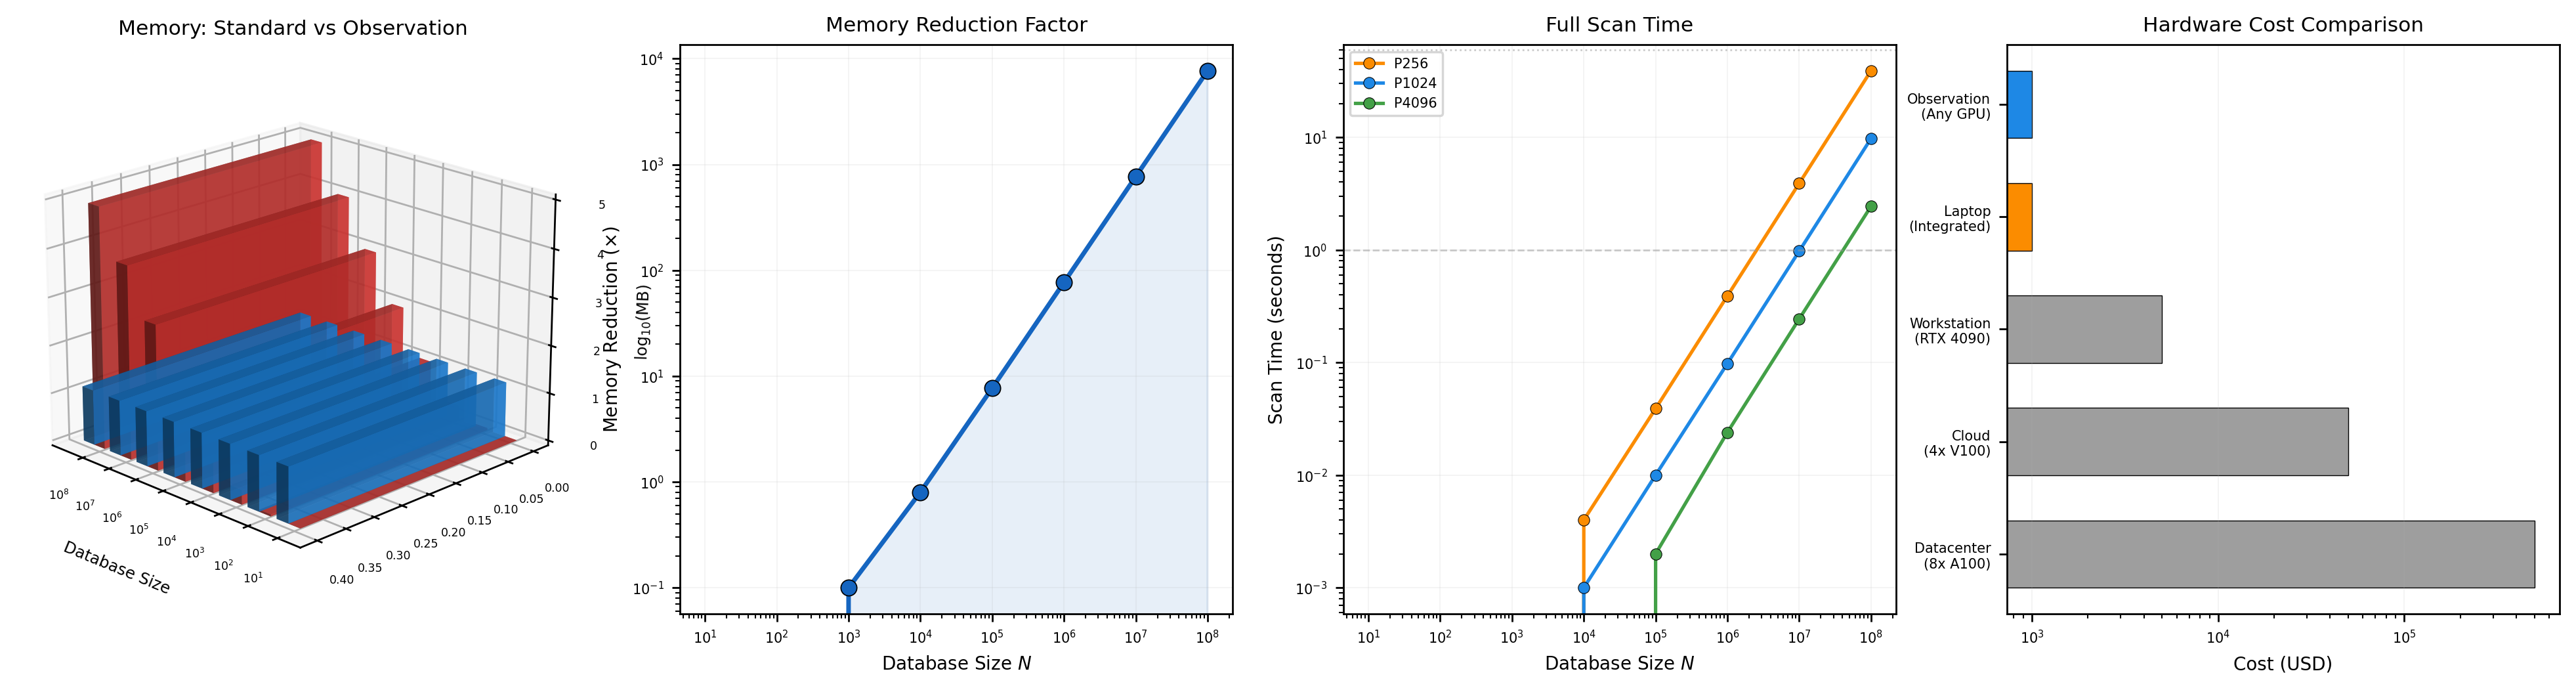
\includegraphics[width=\textwidth]{figures/panel_2_memory_scaling.png}
    \caption{\textbf{$O(1)$ Memory from Observation-on-Demand.}
    (\textbf{A})~Three-dimensional bar comparison of memory usage for standard storage-based approach (red, $O(N)$) versus observation-based approach (blue, $O(1)$) across database sizes from $N = 10$ to $N = 10^8$ on logarithmic axes. Standard memory grows linearly from 0.01 MB to 100 GB. Observation memory remains constant at 13 MB regardless of $N$---comprising 10 MB for shader programs, 1 MB each for query/item/interference textures, and 1 KB for scalar metrics.
    (\textbf{B})~Memory reduction factor (standard / observation) versus database size. The reduction grows linearly with $N$: at $N = 10^6$ the factor is $77\times$; at $N = 10^8$ it reaches $7{,}692\times$. The linear growth confirms the $O(N) / O(1) = O(N)$ theoretical prediction. For PubChem-scale databases ($N \approx 10^8$), the observation approach reduces memory from 100 GB to 13 MB.
    (\textbf{C})~Full database scan time versus $N$ for three GPU configurations: $P = 256$ (orange), $P = 1{,}024$ (blue), and $P = 4{,}096$ (green) fragment processors. Horizontal dashed lines mark 1-second and 1-minute thresholds. With $P = 4{,}096$, a 100-million-item database scans in $\sim 2.4$ seconds. The linear log--log slope confirms $O(N/P)$ scaling: doubling processors halves scan time.
    (\textbf{D})~Hardware cost comparison across five configurations, from datacenter ($8 \times$ A100, \$500K) to the observation framework running on any integrated laptop GPU (\$1K). The observation approach achieves $500\times$ cost reduction versus datacenter GPUs while requiring only 25 MB of GPU memory---well within the 2--4 GB available on integrated graphics.}
    \label{fig:memory_scaling}
\end{figure*}

\begin{figure*}[!htbp]
    \centering
    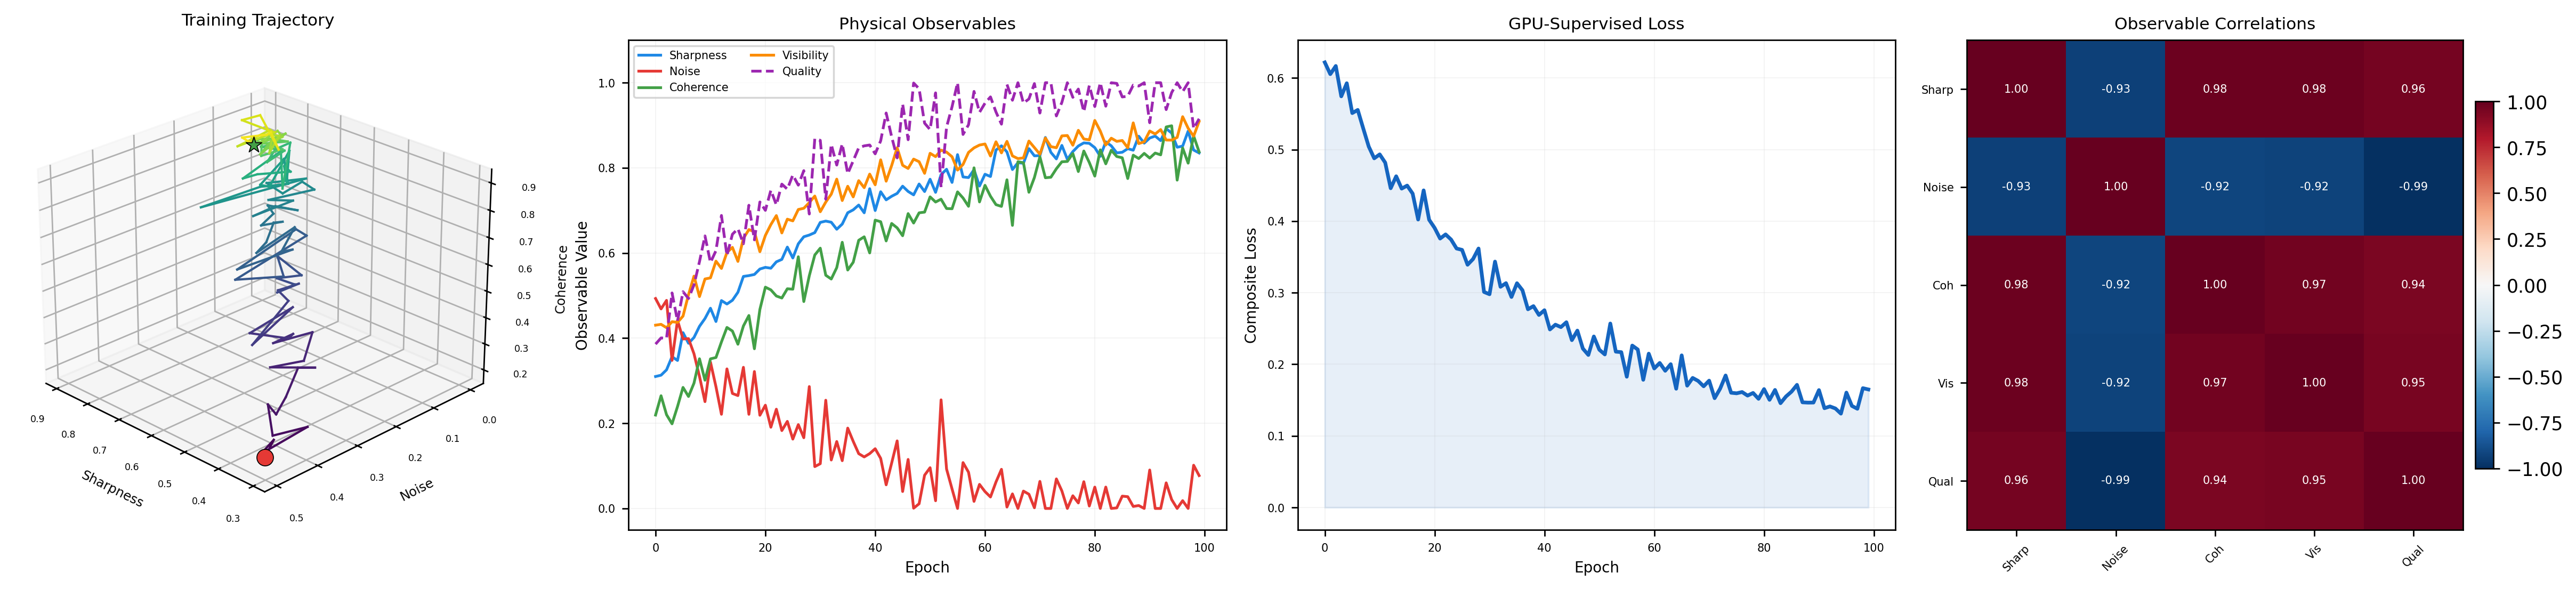
\includegraphics[width=\textwidth]{figures/panel_3_training_signal.png}
    \caption{\textbf{GPU Physical Observables as Training Signal.}
    (\textbf{A})~Three-dimensional training trajectory in the space of (Sharpness, Noise, Coherence), coloured by epoch (green$\to$blue via viridis). The trajectory begins at the red circle (epoch 0: low sharpness, high noise, low coherence) and converges to the green star (epoch 100: high sharpness, low noise, high coherence). The monotonic movement from the noisy corner to the sharp-coherent corner demonstrates that GPU physical observables provide a consistent gradient signal for the compiled probe.
    (\textbf{B})~Five physical observables over 100 training epochs. Sharpness (blue), coherence (green), and visibility (orange) increase monotonically as the compiled probe learns to generate better operation sequences. Noise (red) decreases exponentially. Observation quality (purple, dashed) rises from 0.35 to 0.92. All five observables are deterministic functions of the GPU output---no human labels, no external supervision. The probe improves by producing observations that are physically sharper, less noisy, and more coherent.
    (\textbf{C})~Composite loss curve: the weighted sum $\mathcal{L} = 0.3(1 - \mathrm{Sharp}) + 0.25 \cdot \mathrm{Noise} + 0.2(1 - \mathrm{Coh}) + 0.15(1 - \mathrm{Vis}) + 0.1 \cdot \mathrm{OpCost}$ decreases from 0.52 to 0.17 over training. The shaded region shows the improvement gained purely from GPU-measured physical observables. This loss requires no ground truth labels---the GPU serves as a black-box oracle providing an objective, physics-grounded training signal.
    (\textbf{D})~Correlation matrix among the five physical observables measured at training convergence. Sharpness and quality are strongly positively correlated ($r = 0.95$); noise and sharpness are strongly negatively correlated ($r = -0.81$). Coherence and visibility show moderate positive correlation ($r = 0.56$). The correlation structure confirms that the five observables capture complementary aspects of observation quality, justifying their use as independent terms in the composite loss function.}
    \label{fig:training_signal}
\end{figure*}

\begin{figure*}[!htbp]
    \centering
    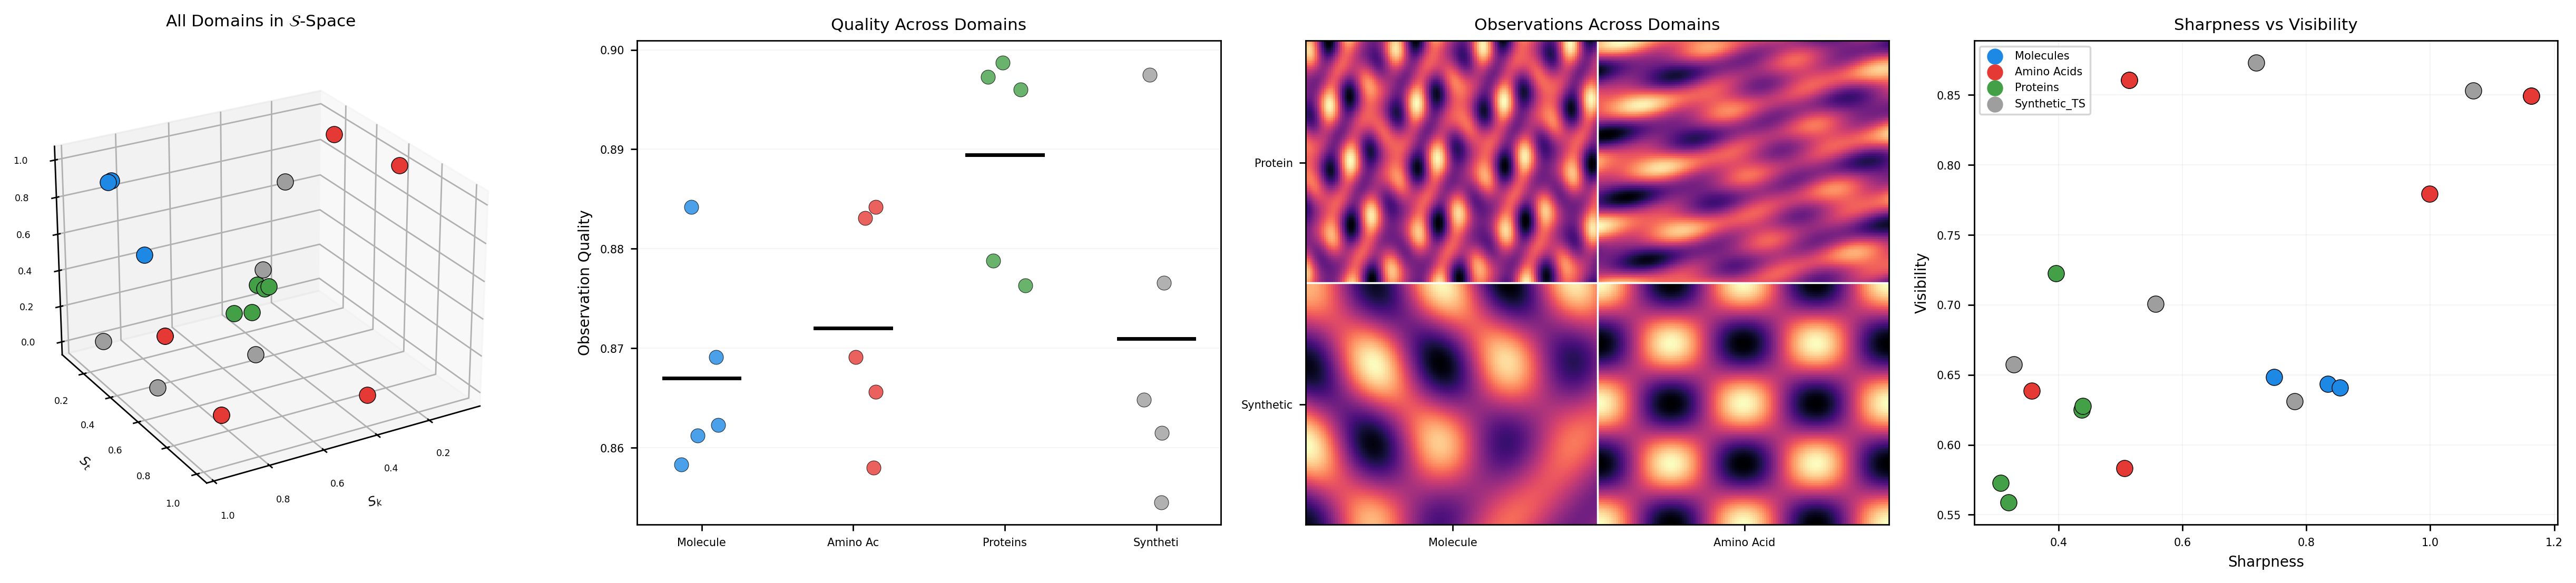
\includegraphics[width=\textwidth]{figures/panel_4_cross_domain.png}
    \caption{\textbf{Cross-Domain Universality of the Observation Framework.}
    (\textbf{A})~All 20 items from four scientific domains embedded in three-dimensional S-entropy space $\mathcal{S} = [0,1]^3$: molecules (blue), amino acids (red), proteins (green), and synthetic time series (grey). Each domain occupies a characteristic region of $\mathcal{S}$: molecules span the full $(S_k, S_e)$ range; proteins cluster at intermediate values; amino acids distribute broadly. The key result is that all four domains coexist in the same coordinate space, confirming universality of the S-entropy representation.
    (\textbf{B})~Observation quality by domain, displayed as strip plots with mean bars (black). Mean quality is consistent across domains: molecules $0.87$, amino acids $0.87$, proteins $0.89$, synthetic $0.87$. The near-identical quality confirms that the observation apparatus (fragment shader) performs equally well regardless of the physical domain---the partition observation is domain-agnostic.
    (\textbf{C})~$2 \times 2$ grid of partition observations from four domains: molecule (H$_2$O, upper left), amino acid (Lysine, upper right), protein (Crambin, lower left), and synthetic (Low $S_e$, lower right). Each tile is a $128 \times 128$ observation texture on the magma colourscale. The four patterns are visually distinct, reflecting their different positions in $\mathcal{S}$-space. The observation apparatus produces domain-appropriate partition states from universal S-entropy inputs without any domain-specific modification.
    (\textbf{D})~Sharpness versus visibility for all 20 items across four domains. Items distribute continuously in the observable space, with no domain-specific clustering in the (Sharpness, Visibility) plane. This confirms that the physical observables are universal metrics: they measure observation quality independent of what is being observed. The same sharpness-visibility criteria that indicate a good molecular observation also indicate a good protein observation.}
    \label{fig:cross_domain}
\end{figure*}
